\documentclass[a4paper,11pt]{article}
\oddsidemargin 0.0cm  
\evensidemargin 0.0cm  
\textwidth 17cm 
\topmargin -1cm 
\textheight 23.5cm
\usepackage{graphicx}
\usepackage{float} 
\usepackage{multimedia}
\usepackage{amsmath,amssymb}
\usepackage{listings}
\usepackage{graphicx} % Allows including images
\usepackage{booktabs} % Allows the use of \toprule, \midrule and \bottomrule in tables

\usepackage{scrextend}
\usepackage{amsfonts}
\usepackage{amsmath,bm}
\usepackage{algorithm}
\usepackage{algorithmic}
\usepackage{graphicx}
\usepackage[round]{natbib}
\lstset{
  numbers=left,   
  firstnumber=1,
  numberfirstline=true,
  language=C, 
  frame=L
  } 

\title{Internship: 2D Geological Storytelling}
\author{Maxime Garcia}
\date{\today}

\begin{document}
\maketitle
\section{Context}

Hand sketching 2D sections of the soil allows geologists to illustrate and validate their hypothesis about recorvering its history. Their assumptions are based on geological knowledge and rules. Moreover by looking at the different layers and faults, the geologist is able to expand or compress the soil to represent what it was like before sedimentation, erosion and tectonic movements.
The resulting drawing is called a reconstitution. \\\\
However this approach is rather limited because it only takes into account the soil history at discrete steps and doesn't necessarily keep the drawing cohesion between two steps.
Recently a new numerical sketching method was proposed [1]. It organizes geological sketches into story trees allowing to compare different interpretations of the soil history . This method allows the geologist to draw over the previous frame in order to help him keep the drawing consitency. It allows also to draw several hypothesis that lead to the same soil configuration and play the animation of those at the same time for comparing them.
However even if such a method can help geologist beeing more consistant and clearer about their hypothesis, we can't visualize the full geological history that a continuous animation can provide.\\\\
Our approach is centered on this continuous animation aspect.
Concretely starting from the 2D current section of the soil we will create automatically a story tree containing all plausible animation scenarios that generated the current soil situation. After generating the tree it will be possible to play the animation starting from the leaves and visualize the forward creation of our 2D current section.


\section{State of the art}

Several continuous animation tools for soil evolution in time are already available.
They work on the assumption that sedimantary layers were in a horizontal configuration at the starting position which is a well used hypothesis in geology. 
With this assumption sofware such as SLAMTec or OptumG2 offer the possibility to mechanically simulate the compression of a sedimental section taking into account friction and erosion.\\\\
The goal of this kind of foward simulation is to validate a reconstruction that had been generated from a present dating 2D section and see if the result coincidates with it. This kind of simulation is configurable by several factors such as the erosion and the friction coefficients.\\\\
Soil reconstructions can be obtained thanks to geometrical tools. Those tools deal with each block (soil section between two faults) one by one and flatten each layer while conserving their respective area. After the flattening operation the user can manually stick the new block to its neighbours with the corresponding layers facing each other. 
Here is an example of reconstitution taken from Chartreuse cut:

\begin{figure}[H]
\centering
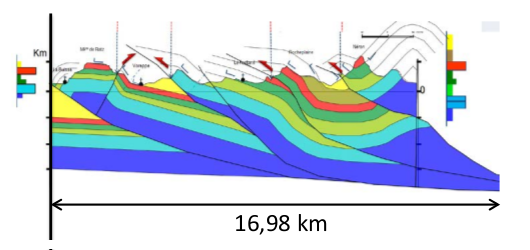
\includegraphics[scale=1]{Wraped_Section.png}
\caption{Current section of Chartreuse soil}
\end{figure}

\begin{figure}[H]
\centering
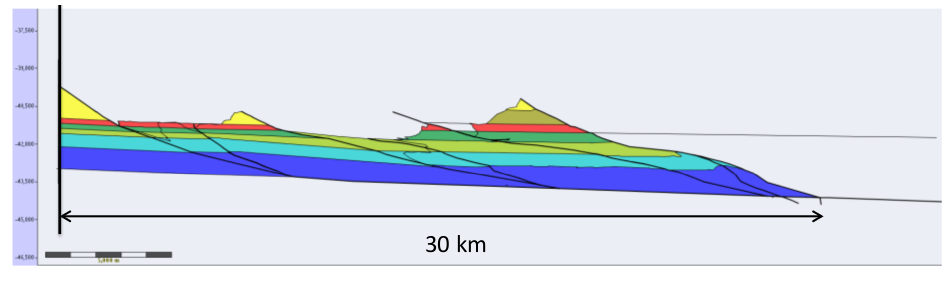
\includegraphics[scale=0.7]{UnWraped_Section.png}
\caption{Reconstitution of Chartreuse soil}
\end{figure}

As this reconstitution is done manually by a geologist it corresponds to a plausible past state of the soil where we can run foward simulation on it to actually compare with the current section and validate it. \\\\
In our case we will take a backward approach: starting from the current 2D section we will simulate the biggest range of plausible transitions beetween this section and the reconstitution.

\section{Our approach}

Unlike forward animation techniques which use a reconstitution and run a mechanical simulation over it, we will run a physical based animation on the current 2D section while proposing all plausible scenarios that lead to it. \\\\
The concatenation of all plausible senarios will take the form of a tree with the the current 2D section as root node.
Each node of the tree will corresponds to a discrete topological event sush as faults, meaning that between two consecutive node levels we will simulate the consequence of this event. Thus the tree banches will correspond to the continuous animation of the soil change caused by the end node event of the branch. \\\\
However discrete geological events are not the only phenomena we have to consider in order to represent all the plausible scenarios. Indeed continuous events such as erosion and sedimentation have to be taken into account. Those events will be integrated into the tree as branches.\\
More phenomena may be added during the internship but we have to be careful to not produce too many scenarios that are not relevent, therefore the number of considered phenomena should be moderated.
However the number of unrelevent scenarios can be reduced by taking into account more geological laws that will restrict node and branch creations.\\
Before genarating the tree we will extract all the information we can from the 2D section, that is to say the number of layers, their age, the already determined eroded zones and so on.\\\\
As geological structures can have a rather complex topology, the 2D section will be presented as a vector graphics complex representation [2] drawn using \textbf{vpaint} software [3]. This data structure has been shown to model all possible incidence relations between vertices, edges and faces in 2D sketches. More structures derivating from vector graphics complex will be implemented in order to take into account the geological aspect of the sketch.\\\\
The animation will be done using a physical model attached into those new structures extending the vector animation complex's one [4] which is used to describe all possible changes in the topology of a vector graphic complex over time.
This physical model will require prior information about several geological parameters that will affect the animation such as materials' density, friction coefficients and others like erosion and sedimentation speeds.


\section{Validation}

The validation will be done by analogic simulations of a real soil with sand boxes. Sedimental layers are disposed in an horizontal manner in order to represent the starting point which corresponds to the reconstruction. Then compression or extension is applied to one or both sides of the box in order to simulate the topological changes in a short time. In addition erosion can be applied by  removing matter from the box. This technique can be used to make unit test in our simulations, for instance when testing only the fault sliding or the erosion effect.

\section{References}

[1] Lidal, Endre Mølster; Natali, Mattia; Patel, Daniel; Hauser, Helwig; Viola, Ivan.
Geological storytelling. Computers \& graphics. 37: 445-459.\\

\noindent[2] Boris Dalstein, Remi Ronfard, Michiel Van De Panne. Vector Graphics Complexes. ACM transactions on
Graphics, Proceedings of ACM SIGGRAPH 2014.\\

\noindent[3] http://www.vpaint.org/ \\

\noindent[4] Boris Dalstein, Rémi Ronfard, Michiel van de Panne. Vector Graphics Animation with Time-Varying Topology.
ACM Transactions on Graphics, 34, 4, Proceedings of ACM SIGGRAPH 2015.


\end{document} 